% Author: Izaak Neutelings (October 2020)
\documentclass[border=3pt,tikz]{standalone}
\usepackage{physics}
\usepackage{tikz}
\usetikzlibrary{angles,quotes} % for pic
\tikzset{>=latex} % for LaTeX arrow head

\colorlet{myred}{red!65!black}
\colorlet{xcol}{blue!70!black}
\colorlet{vcol}{green!70!black}
\colorlet{acol}{red!50!blue!80!black!80}
\tikzstyle{mass}=[line width=0.6,red!30!black,fill=red!40!black!10,rounded corners=1,
                  top color=red!40!black!20,bottom color=red!40!black!10,shading angle=20]
\tikzstyle{vvec}=[->,vcol,very thick,line cap=round]
\tikzstyle{avec}=[->,acol,very thick,line cap=round]


\begin{document}


% POSITIVE ACCELERATION
\def\v{1.6}  % velocity magnitude
\def\a{0.8}  % acceleration magnitude
\def\ang{30} % angle
\begin{tikzpicture}
  \coordinate (O) at (0,0);
  \coordinate (V) at (\ang:\v);
  \coordinate (A) at (\ang:\a);
  \draw[vvec] (O)++(\ang-90:0.1) --++ (V) node[above=2,right=-2] {$\vb{v}$};
  \draw[avec] (O)++(\ang+90:0.1) --++ (A) node[above=0] {$\vb{a}$};
\end{tikzpicture}


% NEGATIVE ACCELERATION
\begin{tikzpicture}
  \coordinate (O) at (0,0);
  \coordinate (V) at (\ang:\v);
  \coordinate (A) at (\ang:\a);
  \draw[vvec] (O)++(\ang-90:0.1) --++ (V) node[above=2,right=-2] {$\vb{v}$};
  \draw[avec] (A)++(\ang+90:0.1) --++ (\ang-180:\a) node[left=-1] {$\vb{a}$};
\end{tikzpicture}


% ANGLED ACCELERATION
\begin{tikzpicture}
  \coordinate (O) at (0,0);
  \coordinate (V) at (10:\v);
  \coordinate (A) at (60:\a);
  \draw[vvec] (O) --++ (V) node[right=-2] {$\vb{v}$};
  \draw[avec] (O) --++ (A) node[left=2] {$\vb{a}$};
  \draw pic["$\theta$",draw=black,angle radius=14,angle eccentricity=1.4] {angle=V--O--A};
\end{tikzpicture}


% ANGLED ACCELERATION - break down
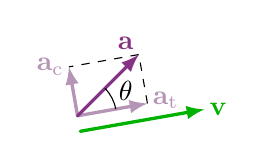
\begin{tikzpicture}
  \def\v{1.6}   % velocity magnitude
  \def\a{1.1}   % acceleration magnitude
  \def\angv{10} % angle velocity
  \def\anga{45} % angle acceleration
  \coordinate (O) at (0,0);
  \coordinate (V) at (\angv:\v);
  \coordinate (A) at (\anga:\a);
  \coordinate (AT) at (\angv:{\a*cos(\anga-\angv)});
  \coordinate (AC) at (\angv+90:{\a*sin(\anga-\angv)});
  \draw[vvec] (O)++(\angv-90:0.2) --++ (V) node[right=-2] {$\vb{v}$};
  \draw[dashed] (AT) -- (A) -- (AC);
  \draw[avec,acol!80!black!50] (O) -- (AT) node[above=1,right=-2] {$\vb{a}_\mathrm{t}$};
  \draw[avec,acol!80!black!50] (O) -- (AC) node[left=-2] {$\vb{a}_\mathrm{c}$};
  \draw[avec] (O) --++ (A) node[above left=-2] {$\vb{a}$};
  \draw pic["$\theta$",draw=black,angle radius=14,angle eccentricity=1.4] {angle=V--O--A};
\end{tikzpicture}


% ANGLED ACCELERATION - opposite
\begin{tikzpicture}
  \coordinate (O) at (0,0);
  \coordinate (V) at (10:\v);
  \coordinate (A) at (160:\a);
  \draw[dashed] (O) --++ (-170:0.4*\v);
  \draw[vvec] (O) --++ (V) node[right=-2] {$\vb{v}$};
  \draw[avec] (O) --++ (A) node[left=2] {$\vb{a}$};
  \draw pic["$\theta$",draw=black,angle radius=9,angle eccentricity=1.65] {angle=V--O--A};
\end{tikzpicture}


% POSITIVE ANGULAR ACCELERATION
\begin{tikzpicture}
  \coordinate (O) at (0,0);
  \coordinate (V) at (\ang:\v);
  \coordinate (A) at (\ang:\a);
  \draw[vvec] (O)++(\ang-90:0.1) --++ (V) node[above=2,right=-2] {$\vb*{\omega}$};
  \draw[avec] (O)++(\ang+90:0.1) --++ (A) node[above=0] {$\vb*{\alpha}$};
\end{tikzpicture}


% NEGATIVE ANGULAR ACCELERATION
\begin{tikzpicture}
  \coordinate (O) at (0,0);
  \coordinate (V) at (\ang:\v);
  \coordinate (A) at (\ang:\a);
  \draw[vvec] (O)++(\ang-90:0.1) --++ (V) node[above=2,right=-2] {$\vb*{\omega}$};
  \draw[avec] (A)++(\ang+90:0.1) --++ (\ang-180:\a) node[left=-1] {$\vb*{\alpha}$};
\end{tikzpicture}


% ANGLED ANGULAR ACCELERATION
\begin{tikzpicture}
  \coordinate (O) at (0,0);
  \coordinate (V) at (10:\v);
  \coordinate (A) at (60:\a);
  \draw[vvec] (O) --++ (V) node[right=-2] {$\vb*{\omega}$};
  \draw[avec] (O) --++ (A) node[left=2] {$\vb*{\alpha}$};
  \draw pic["$\theta$",draw=black,angle radius=14,angle eccentricity=1.4] {angle=V--O--A};
\end{tikzpicture}


\end{document}